% Section content template for individual Educative lessons
% This file contains the actual content for a specific section
% Generated from Educative API section content

% Section: Getting Ready: The ESPNcricinfo System
% Section ID: 5701411636772864
% Section Slug: getting-ready-the-espncricinfo-system
% Generated: 2025-12-14T13:32:11.838110

\subsection{Problem definition}\label{8t9y4PhhhzAHjxEhcwrhA}
\\
\textbf{ESPNcricinfo} is a comprehensive cricket management and broadcasting system that offers real-time and historical data for cricket matches, players, teams, and tournaments. It supports various formats, including Test, ODI, and T20 matches. The platform is designed for multiple stakeholders, admins, coaches, umpires, and commentators, each with distinct roles and responsibilities.
\\
The system enables ball-by-ball tracking of match events, including wickets, scores, and live commentary, providing an engaging experience for viewers and analysts. The admin can add or update all statistics related to players, teams, and matches, ensuring data accuracy and completeness.
\\
ESPNcricinfo also handles tournament management, allowing the admin to add and modify tournaments, assign stadiums and match personnel, and manage team participation. For each tournament, coaches can select a squad of players to represent the team. From this squad, the playing eleven can be chosen for each match.
\\
Additionally, the system maintains points tables, match results, and complete historical data for previous tournaments and games. It includes features for publishing cricket news and updates, managed by the admin or coaches, and provides tools for commentators to input or update commentary during live matches.

\begin{figure}[htbp]
 \centering
 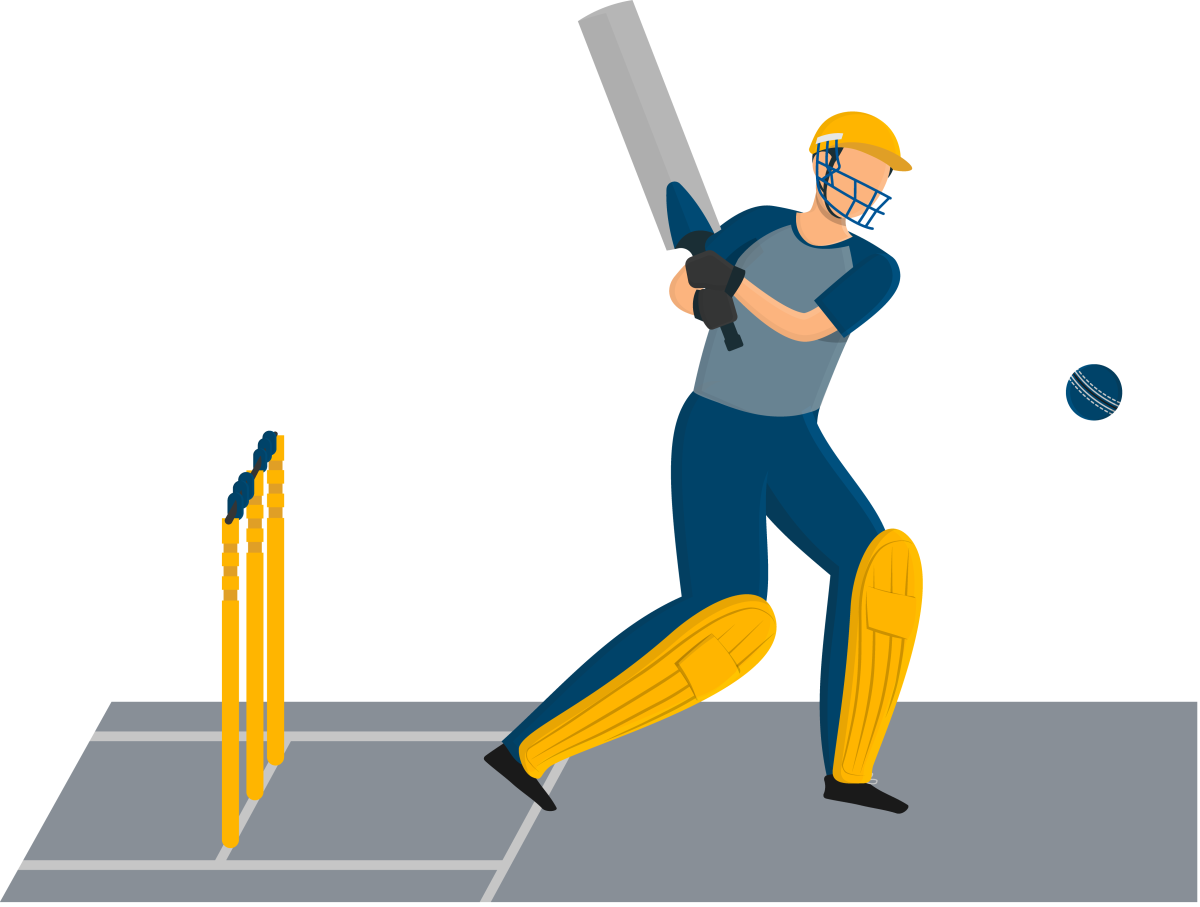
\includegraphics[width=0.5\textwidth]{Images/chapter_26/section_5701411636772864/6548350959878144.png}
 
\end{figure}

\subsection{Expectations from the interviewee}\label{8mWjBBkzQ_msT38LKJm8y-2}
\\
ESPNcricinfo is a role-based cricket management system that supports match operations, tournament setup, and the handling of real-time data. During the interview, you are expected to clearly understand the system's actors, their responsibilities, and the use cases that drive the system. You should ask relevant questions that help clarify the system's functional and operational behavior.

\subsubsection{Player, team, and match statistics}\label{LrV9x8wla_x0ipgAWFefy}
\\
The system must accurately track player, team, and match statistics.

\begin{itemize}
\item
\protect\phantomsection\label{bCwLxe3cptwDUQm87YifE}
How are player statistics updated---manually by the admin or through automation?
\item
\protect\phantomsection\label{M_1MgQbbCmSjfbcqcG1jn}
What statistical detail is required (e.g., runs, wickets, strike rate)?
\item
\protect\phantomsection\label{Sk-d-o0Lr7V3scGgj2KGa}
Should stats be updated after every ball, inning, or match?
\end{itemize}

\subsubsection{Match formats and match management}\label{29VSaRKtpoMuMItGXEwF_}
\\
The system must support all three formats: Test, ODI, and T20.

\begin{itemize}
\item
\protect\phantomsection\label{PFEOujtOW1qMHPuEM-YQi}
Are there format-specific rules that need to be encoded in the system?
\item
\protect\phantomsection\label{0WjJ2NnvCw3odMPNW8c6v}
Should match duration or innings logic be handled differently based on format?
\end{itemize}

\subsubsection{Squad submission for tournaments}\label{F3fzr1iSpc-e4wJjOtY5g}
\\
Each team must submit a tournament squad in advance.

\begin{itemize}
\item
\protect\phantomsection\label{w3Wm1ASJh__urW9JoeFAq}
Who is responsible for submitting the squad?
\item
\protect\phantomsection\label{H9-gM1jqigPrFy6eAhqRb}
Can a coach modify the squad after it has been submitted, and under what conditions?
\end{itemize}

\subsubsection{Admin operations}\label{_ERYWz5WK1_YzwsmCbUD5}
\\
The admin oversees the creation and management of all entities in the system.

\begin{itemize}
\item
\protect\phantomsection\label{BnbOR0EJdQgJld3RtFIQn}
What validations are needed when adding matches, players, or teams?
\item
\protect\phantomsection\label{wHJXi6b1hUqzAnRwvFhc0}
How are stadiums and match personnel assigned?
\item
\protect\phantomsection\label{Lwr90GTbrcR5QZKdnhkE2}
Is there a review or approval step before updates go live?
\end{itemize}

\subsection{Design approach}\label{jm1e21p9FThwea5VKBcnN}
\\
We'll design Cricinfo using the bottom-up approach. For this purpose, we will follow the steps below:

\begin{itemize}
\item
\protect\phantomsection\label{QX-Zui5p7LPdlh9JYvzN4}
Identify and design the smallest components, like a ball and a run.
\item
\protect\phantomsection\label{5RQOXIKhFR2AnHkRk1iFi}
Use these small components to design larger components, such as an over, a team, and an umpire.
\item
\protect\phantomsection\label{0g7y3rcGDHAvhxJyUcPRh}
Repeat the steps above until we design the complete ESPNcricinfo platform.
\end{itemize}

\subsection{Design pattern~}\label{WfezANT5h4UD7KowbRqQH}
\\
During an interview, discussing the design patterns that ESPNcricinfo falls under is always a good practice. Stating the design patterns gives the interviewer a positive impression and shows that the interviewee is well-versed in the advanced concepts of object-oriented design.
\\
Try to answer the following question. If you are not familiar with design patterns, don't worry! You can learn about them by asking, ``Define design patterns.''

\textbf{Question:}

Which design pattern(s) should be used to design the Cricinfo system? Please elaborate on your choice(s).

Let's explore the requirements for ESPNcricinfo in the next lesson.

\subsection{}\label{M9-YDfJ3O0hpngktvq5Uz}

% End of section content